\begin{figure*}[t]
\centering
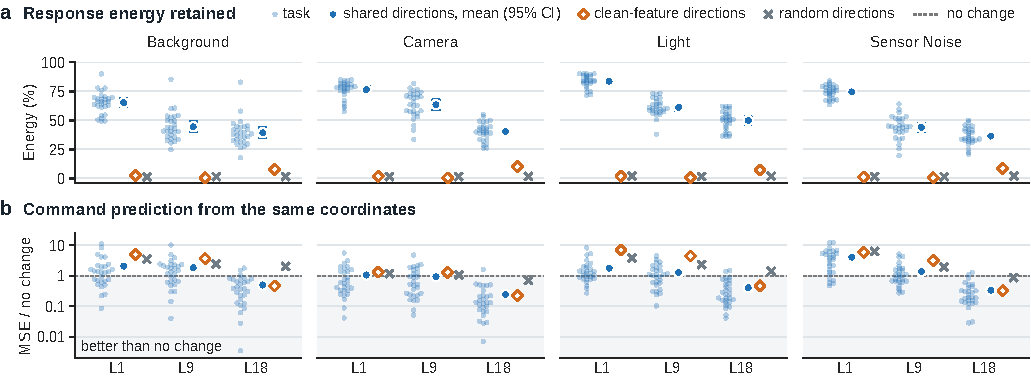
\includegraphics[width=\textwidth]{revised_figures/figure3_geometry_v3.pdf}
\caption{\textbf{Shared directions retain far more of an unseen response than the controls; the commands are predicted best at the last layer.} Both panels: 404 pairs on 28 tasks; each fit leaves out the test tasks and the test family. For the shared directions, small dots are tasks and large dots their means; diamonds and crosses are the two controls. (a) Share of the response energy that 16 directions retain; the means carry pointwise 95\% intervals. (b) Error of a linear readout that predicts the change in the first five commands from the same 16 coordinates, divided by the family-mean error of predicting that the commands do not change; large markers are ratios of task means. Below 1 (shaded), the readout beats predicting no change. Paired comparisons: Supplement, Secs.~S3.4 and~S14.}
\label{fig:token-structure}
\end{figure*}
